\documentclass[aspectratio=169]{beamer}
\usepackage[T2A]{fontenc} % Без этого с компилятором pdflatex не работает
\usepackage[utf8]{inputenc} % Без этого с компилятором pdflatex не работает
\usepackage[russian]{babel} % Без этого с компилятором pdflatex не работает
\usepackage{graphicx} % Для вставки изображений
\usetheme{Madrid} 
\usecolortheme{seahorse}
\setbeamertemplate{footline}{%
	\leavevmode%
	\hbox{%
		\begin{beamercolorbox}[wd=.6\paperwidth,ht=2.5ex,dp=1ex,left]{palette primary}%
			\hspace{0.5em}Студенты АлтГТУ, группа 8 ПИ-51
		\end{beamercolorbox}%
		\begin{beamercolorbox}[wd=.4\paperwidth,ht=2.5ex,dp=1ex,right]{palette primary}%
			\insertshortdate\hspace{1em}\insertframenumber/\inserttotalframenumber\hspace{0.5em}
		\end{beamercolorbox}%
	}%
	\vskip0pt%
}

\title{Оценка реализации устойчивой к сбоям real-time OS}
\subtitle{Применение Erlang в такого рода задачах}

\author{
	Студенты АлтГТУ, группа 8 ПИ-51\\
	Бельш А.Е.\\
	Воробьев К.В.\\
	Мэн Ч.\\
	Ошурков Н.А.
}

\date{2026 г.}

\begin{document}
	
	\frame{\titlepage}
	\begin{frame}{Отказоустойчивость в Erlang}
	\textbf{Erlang} — язык для распределённых систем с высокой надёжностью.
	
	\vspace{0.5em}
	Ключевые цели:
	\begin{itemize}
		\item Система должна работать при сбоях отдельных частей;
		\item Минимизация простоя;
		\item Автоматическое восстановление.
	\end{itemize}
	
	\vspace{0.5em}
	Основной подход: \textbf{“Let it crash”}
\end{frame}
	\begin{frame}{Модель процессов Erlang: свойства}
	\textbf{Особенности процессов:}
	\vspace{0.5em}
	\begin{itemize}
		\item Легковесные (тысячи/миллионы процессов);
		\item Изолированная память;
		\item Нет разделяемой памяти (shared memory);
		\item Каждый процесс выполняется независимо.
	\end{itemize}
	\vspace{0.8em}
	\textbf{Вывод:} процессы не влияют напрямую друг на друга, что повышает отказоустойчивость.
\end{frame}
	\begin{frame}{Модель процессов Erlang: обмен сообщениями}
	\begin{flushleft}
		\textbf{Идея:} процессы не разделяют память и взаимодействуют только через передачу сообщений.
	\end{flushleft}
	\vspace{0.8em}
	\begin{center}
		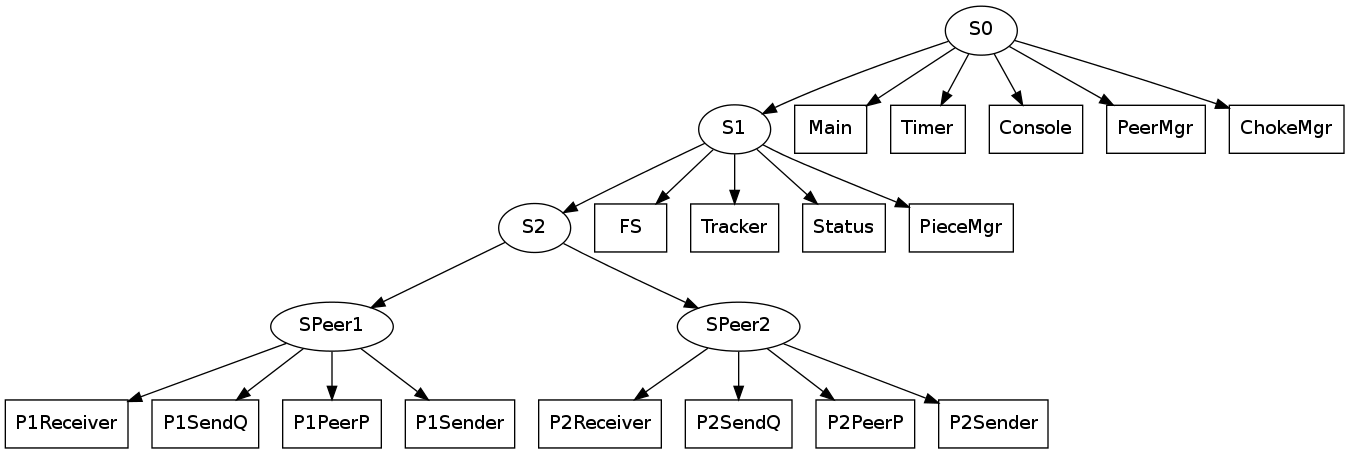
\includegraphics[width=0.75\textwidth]{process_model.png}
	\end{center}
\end{frame}
	\begin{frame}{Принцип “Let it crash”}
	\begin{itemize}
		\item Ошибки не обрабатываются вручную в каждом месте;
		\item Процесс при сбое завершается;
		\item Восстановление выполняет supervisor.
	\end{itemize}
	
	\vspace{0.5em}
	\textbf{Идея:} проще перезапустить корректно, чем исправлять сложное состояние.
\end{frame}
	\begin{frame}{Дерево надзора (Supervision Tree)}
	\begin{flushleft}
		\textbf{Идея:} система строится как дерево процессов, где часть процессов контролирует другие.
	\end{flushleft}
	\vspace{0.8em}
	\centering
	\begin{tabular}{|c|c|c|}
		\hline
		\textbf{Тип процесса} & \textbf{Функция} & \textbf{Поведение при сбое} \\
		\hline
		Worker & Выполняет задачу & Перезапускается supervisor’ом \\
		\hline
		Supervisor & Контролирует worker’ов & Перезапускает процессы \\
		\hline
	\end{tabular}
	\vspace{1em}
	\begin{flushleft}
		\textbf{Свойство:} система самовосстанавливается за счёт перезапуска упавших процессов.
	\end{flushleft}
\end{frame}
	\begin{frame}{OTP (Open Telecom Platform)}
	OTP предоставляет готовые механизмы устойчивости:
	
	\begin{itemize}
		\item Стандартизированные процессы;
		\item Стратегии восстановления:
		\begin{itemize}
			\item one\_for\_one
			\item one\_for\_all
			\item rest\_for\_one
		\end{itemize}
		\item Шаблоны распределённых систем.
	\end{itemize}
\end{frame}
	\begin{frame}{Связь с real-time OS}
	
	Идеи Erlang применимы в RTOS:
	
	\begin{itemize}
		\item Изоляция задач (как процессы Erlang);
		\item Восстановление без остановки системы;
		\item Предотвращение каскадных отказов.
	\end{itemize}
	
	\vspace{0.5em}
	
	В контексте POK kernel:
	\begin{itemize}
		\item Задачи = Процессы;
		\item Планировщик = Supervisor-подобная логика.
	\end{itemize}
\end{frame}
	\begin{frame}{Промежуточные выводы}
	\begin{itemize}
		\item Erlang реализует отказоустойчивость через изоляцию процессов и супервизоры;
		\item Ошибки не предотвращаются полностью, а локализуются и приводят к перезапуску;
		\item Система продолжает работу даже при сбоях отдельных компонентов;
		\item Подход особенно эффективен в распределённых и real-time системах.
	\end{itemize}
	\vspace{0.8em}
	\textbf{Главная идея:} стабильность достигается за счёт контролируемых (управляемых) локальных сбоев и быстрого восстановления.
\end{frame}
	
\end{document}
